\documentclass[journal,12pt,twocolumn]{IEEEtran}

\usepackage{setspace}
\usepackage{gensymb}
\singlespacing
\usepackage{amsmath}
\usepackage{amsthm}
\usepackage{comment}
\usepackage{mathrsfs}
\usepackage{txfonts}
\usepackage{stfloats}
\usepackage{bm}
\usepackage{cite}
\usepackage{cases}
\usepackage{subfig}
\usepackage{blkarray}

\usepackage{longtable}
\usepackage{multirow}

\usepackage{enumitem}
\usepackage{mathtools}
\usepackage{steinmetz}
\usepackage{tikz}
\usepackage{circuitikz}
\usepackage{verbatim}
\usepackage{tfrupee}
\usepackage[breaklinks=true]{hyperref}
\usepackage{graphicx}
\usepackage{tkz-euclide}

\usetikzlibrary{calc,math}
\usetikzlibrary{automata, positioning}
\usepackage{listings}
    \usepackage{color}                                            %%
    \usepackage{array}                                            %%
    \usepackage{longtable}                                        %%
    \usepackage{calc}                                             %%
    \usepackage{multirow}                                         %%
    \usepackage{hhline}                                           %%
    \usepackage{ifthen}                                           %%
    \usepackage{lscape}     
\usepackage{multicol}
\usepackage{chngcntr}

\DeclareMathOperator*{\Res}{Res}

\renewcommand\thesection{\arabic{section}}
\renewcommand\thesubsection{\thesection.\arabic{subsection}}
\renewcommand\thesubsubsection{\thesubsection.\arabic{subsubsection}}

\renewcommand\thesectiondis{\arabic{section}}
\renewcommand\thesubsectiondis{\thesectiondis.\arabic{subsection}}
\renewcommand\thesubsubsectiondis{\thesubsectiondis.\arabic{subsubsection}}


\hyphenation{op-tical net-works semi-conduc-tor}
\def\inputGnumericTable{}                                 %%

\lstset{
%language=C,
frame=single, 
breaklines=true,
columns=fullflexible
}

\begin{document}

\newcommand{\BEQA}{\begin{eqnarray}}
\newcommand{\EEQA}{\end{eqnarray}}
\newcommand{\define}{\stackrel{\triangle}{=}}
\bibliographystyle{IEEEtran}
\raggedbottom
\setlength{\parindent}{0pt}
\providecommand{\mbf}{\mathbf}
\providecommand{\pr}[1]{\ensuremath{\Pr\left(#1\right)}}
\providecommand{\qfunc}[1]{\ensuremath{Q\left(#1\right)}}
\providecommand{\sbrak}[1]{\ensuremath{{}\left[#1\right]}}
\providecommand{\lsbrak}[1]{\ensuremath{{}\left[#1\right.}}
\providecommand{\rsbrak}[1]{\ensuremath{{}\left.#1\right]}}
\providecommand{\brak}[1]{\ensuremath{\left(#1\right)}}
\providecommand{\lbrak}[1]{\ensuremath{\left(#1\right.}}
\providecommand{\rbrak}[1]{\ensuremath{\left.#1\right)}}
\providecommand{\cbrak}[1]{\ensuremath{\left\{#1\right\}}}
\providecommand{\lcbrak}[1]{\ensuremath{\left\{#1\right.}}
\providecommand{\rcbrak}[1]{\ensuremath{\left.#1\right\}}}
\theoremstyle{remark}
\newtheorem{rem}{Remark}
\newcommand{\sgn}{\mathop{\mathrm{sgn}}}
\providecommand{\abs}[1]{\vert#1\vert}
\providecommand{\res}[1]{\Res\displaylimits_{#1}} 
\providecommand{\norm}[1]{\lVert#1\rVert}
%\providecommand{\norm}[1]{\lVert#1\rVert}
\providecommand{\mtx}[1]{\mathbf{#1}}
\providecommand{\mean}[1]{E[ #1 ]}
\providecommand{\fourier}{\overset{\mathcal{F}}{ \rightleftharpoons}}
%\providecommand{\hilbert}{\overset{\mathcal{H}}{ \rightleftharpoons}}
\providecommand{\system}{\overset{\mathcal{H}}{ \longleftrightarrow}}
	%\newcommand{\solution}[2]{\textbf{Solution:}{#1}}
\newcommand{\solution}{\noindent \textbf{Solution: }}
\newcommand{\cosec}{\,\text{cosec}\,}
\providecommand{\dec}[2]{\ensuremath{\overset{#1}{\underset{#2}{\gtrless}}}}
\newcommand{\myvec}[1]{\ensuremath{\begin{pmatrix}#1\end{pmatrix}}}
\newcommand{\mydet}[1]{\ensuremath{\begin{vmatrix}#1\end{vmatrix}}}
\numberwithin{equation}{subsection}
\makeatletter
\@addtoreset{figure}{problem}
\makeatother
\let\StandardTheFigure\thefigure
\let\vec\mathbf
\renewcommand{\thefigure}{\theproblem}
\def\putbox#1#2#3{\makebox[0in][l]{\makebox[#1][l]{}\raisebox{\baselineskip}[0in][0in]{\raisebox{#2}[0in][0in]{#3}}}}
     \def\rightbox#1{\makebox[0in][r]{#1}}
     \def\centbox#1{\makebox[0in]{#1}}
     \def\topbox#1{\raisebox{-\baselineskip}[0in][0in]{#1}}
     \def\midbox#1{\raisebox{-0.5\baselineskip}[0in][0in]{#1}}
\vspace{3cm}
\title{Assignment 4- Probability and Random Variables}
\author{Songa Kotesh Satvik}
\maketitle
\newpage
\bigskip
\renewcommand{\thefigure}{\theenumi}
\renewcommand{\thetable}{\theenumi}
Download all python codes from 
\begin{lstlisting}
https://github.com/KoteshSatvik/AI1103-Probability_and_Random_Variables/tree/main/Assignment-4/codes
\end{lstlisting}
%
and latex-tikz codes from 
%
\begin{lstlisting}
https://github.com/KoteshSatvik/AI1103-Probability_and_Random_Variables/blob/main/Assignment-4/Assignment4.tex
\end{lstlisting}
\section{\textbf{Gate 2016 (cs-set 1) Q:}29}
Consider the experiment with the following steps.
\begin{enumerate}
\item  Flip a coin twice.
\item If the outcomes are (TAILS, HEADS) then output Y and stop.
\item If the outcomes are either (HEADS, HEADS) or (HEADS, TAILS), then output N and stop.
\item If the outcomes are (TAILS, TAILS), then go to Step 1.
\end{enumerate}
The probability that the output of the experiment is Y is (upto two decimal places)......
\section{\textbf{Solution}}
Given a fair coin is flipped twice.\\
Let us define a Markov chain with states \{1,2,3,4\}, such that 
\begin{table}[hbt!]
\resizebox{\columnwidth}{!}{
\begin{tabular}{|c|l|}
\hline
\textbf{State} & \multicolumn{1}{c|}{\textbf{Events}}                     \\ \hline
1                 & Event of tossing a fair coin twice                           \\ \hline
2                 & Event of obtaining 'N' as the output                         \\ \hline
3                 & Event of obtaining 'Y' as the output                         \\ \hline
4                 & Event of obtaining (TAIL,TAIL) as the output                 \\ \hline
\end{tabular}
}
\caption{Representation of different events}
\label{table:1}
\end{table}
\\We know that when a fair coin is tossed,
\begin{align}
    \pr{\text{HEAD}} &=  1/2 \text{ and }\\
    \pr{\text{TAIL}} &=  1/2.
\end{align}
Then, \\
\textbf{Markov chain diagram :}\\
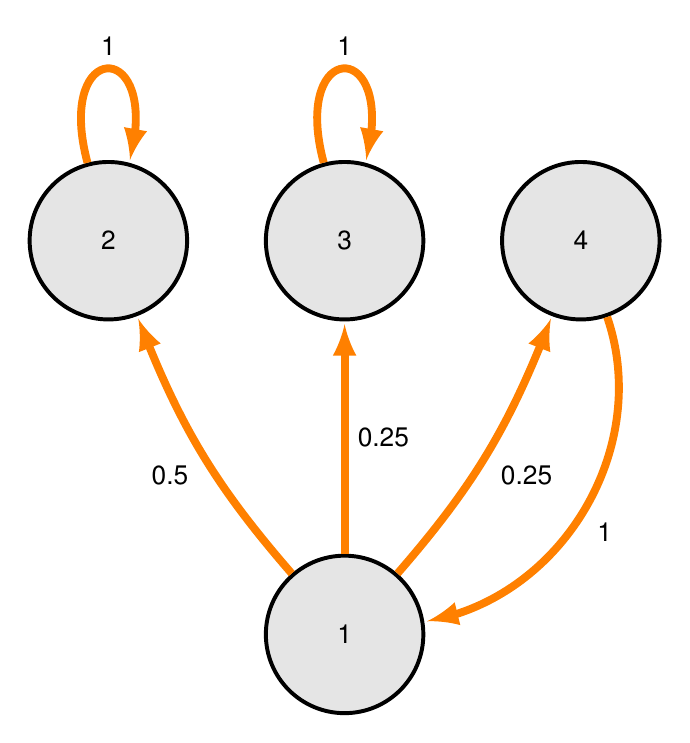
\begin{tikzpicture}[font=\sffamily]

        % Setup the style for the states
        \tikzset{node style/.style={state, 
                                    minimum width=2cm,
                                    line width=0.5mm,
                                    fill=gray!20!white}}

        % Draw the states
        \node[node style] at (1, 0)     (2)     {2};
        \node[node style] at (4, 0)     (3)     {3};
        \node[node style] at (7, 0)     (4)     {4};
        \node[node style] at (4, -5)    (1)     {1};
        
        % Connect the states with arrows
        \draw[every loop,
              auto=right,
              line width=1mm,
              >=latex,
              draw=orange,
              fill=orange]
            (1)     edge[bend left=10, auto=left]  node {0.5} (2)
            (1)     edge                node {0.25} (3)
            (1)     edge[bend right=10, auto=right] node {0.25} (4)
            (4)     edge[bend left=50, auto=left]            node {1} (1)
            (3)     edge[loop above]                node {1} (3)
            (2)     edge[loop above]                node {1} (2)
            ;
\end{tikzpicture}

The state transition matrix (P) for the Markov chain is
\begin{align}
\label{1}
    P=\begin{blockarray}{ccccc}
& 1 & 2 & 3 & 4 \\
\begin{block}{c[cccc]}
  1 & 0 & \frac{1}{2} & \frac{1}{4}  & \frac{1}{4}  \\
  2 & 0 & 1 & 0 & 0 \\
  3 & 0 & 0 & 1 & 0 \\
  4 & 1 & 0 & 0 & 0 \\
\end{block}
\end{blockarray}
\end{align}
By the definition of transient and absorbing states, we can say that 1,4 are transient states whereas 2,3 are absorbing.\\
Then, the canonical form of the transition matrix is,
\begin{align}
\label{2}
    P=\begin{blockarray}{ccccc}
& 2 & 3 & 1 & 4 \\
\begin{block}{c[cc|cc]}
  2 & 1 & 0 & 0 & 0  \\
  3 & 0 & 1 & 0 & 0 \\ 
  \cline{2-5}
  1 & \frac{1}{2} & \frac{1}{4} & 0 & \frac{1}{4} \\
  4 & 0 & 0 & 1 & 0 \\
\end{block}
\end{blockarray}
\end{align}

The canonical form divides the transition matrix into four sub-matrices based on the states as listed below.\\
\begin{blockarray}{ccc}
& \text{Absorbing} & \text{Non-Absorbing} \\
\begin{block}{c[c|c]}
  \text{Absorbing} & I & O \\
  \cline{2-3}
  \text{Non-Absorbing} & A & B \\
  \end{block}
\end{blockarray}
\\where,
\begin{table}[hbt!]
\centering
\begin{tabular}{|c|c|}
    \hline
    \textbf{Variable} & \textbf{Type of Matrix} \\
    \hline
    $I$ & Identity matrix\\
    \hline
    $O$ & Zero matrix\\
    \hline
    $A,B$ & Some matrices\\
    \hline
\end{tabular}
\caption{Representation of different matrices}
\label{table:2}
\end{table}
\\and From \eqref{2},
\begin{align}
\label{3}
    A=\begin{bmatrix}
    \frac{1}{2} & \frac{1}{4}\\
    0 & 0\\
    \end{bmatrix},
    B=\begin{bmatrix}
    0 & \frac{1}{4} \\
    1 & 0 \\
    \end{bmatrix}
\end{align}
The fundamental matrix F for the absorbing Markov chain is defined as 
\begin{align}
    F &=(I-B)^{-1} \label{4}\\
\shortintertext{Then,  }
    F &= \begin{bmatrix}
    1 & -\frac{1}{4} \\
    -1 & 1 \\ 
    \end{bmatrix}^{-1} \\
    \implies F &= \begin{bmatrix}
               1.33 & 0.33 \\
               1.33 & 1.33 \\ 
               \end{bmatrix}\\
\shortintertext{Therefore,}
    FA &= \begin{bmatrix}
    0.67 & 0.33 \\
    0.67 & 0.33 \\ 
    \end{bmatrix}
    \end{align}
Then the limiting matrix for the markov chain is 
\begin{align}
\label{5}
    \bar P&=\begin{bmatrix}
    I & O\\
    FA & O\\
    \end{bmatrix}
\end{align}
where the element $p_{ij}$ of $\bar P$ represents the probability of absorption in state j, when the initial state is i.
\begin{align}
  \therefore \bar P&=\begin{blockarray}{ccccc}
                  & 2 & 3 & 1 & 4 \\
                  \begin{block}{c[cccc]}
                  2 & 1 & 0 & 0 & 0  \\
                  3 & 0 & 1 & 0 & 0 \\ 
                  1 & 0.67 & 0.33 & 0 & 0 \\
                  4 & 0.67 & 0.33 & 0 & 0 \\
                \end{block}
                \end{blockarray}  
\end{align}
Therefore,
\begin{align}
    \text{ Req. Probability }= p_{13} = 0.33
\end{align}
\end{document}
